% Appendix A

\chapter{Extension of the Results Section} % Main appendix title

\label{AppendixA} % For referencing this appendix elsewhere, use \ref{AppendixA}

\lhead{Appendix A. \emph{Extension of the Results Section}} % This is for the header on each page - perhaps a shortened title

\section{Manual classification of the poses of users}

To analyze the dataset used in Chapter \ref{Chapter4}, each of the poses for the different users was plotted. The entries were divided in 3 classes: \emph{pointing right}, \emph{pointing left}, \emph{pointing forward}. The classes were subvidided in sub-classes, depending on the position of both arms, as can be seen in the following tables.

The tables are divided by pose, the first one representing all \emph{pointing right} entries, the second \emph{pointing left} and the third \emph{pointing forward}. The two first columns represent the pointing hand for that pose, and what the user is doing with the other hand. The third column is the number of the users that are posing with that same disposition of arms. The fourth is a Figure example to show the disposition with the 3D data.

\begin{table}
  [h] \caption{Users pointing \emph{right}}
  \renewcommand{\arraystretch}{2}
  \begin{tabular}
      {|l|l|p{4cm}|p{4cm}|} \hline Pointing hand  & Other hand & Users & Figure Example \\
      \hline 
      RIGHT & Hanging & 
      1,2,5,7,8,11,12,13,14,15,\newline
      16,17,18,19,20,21,23,25,\newline26,27,28,29,30 & \parbox[c]{1em}{
      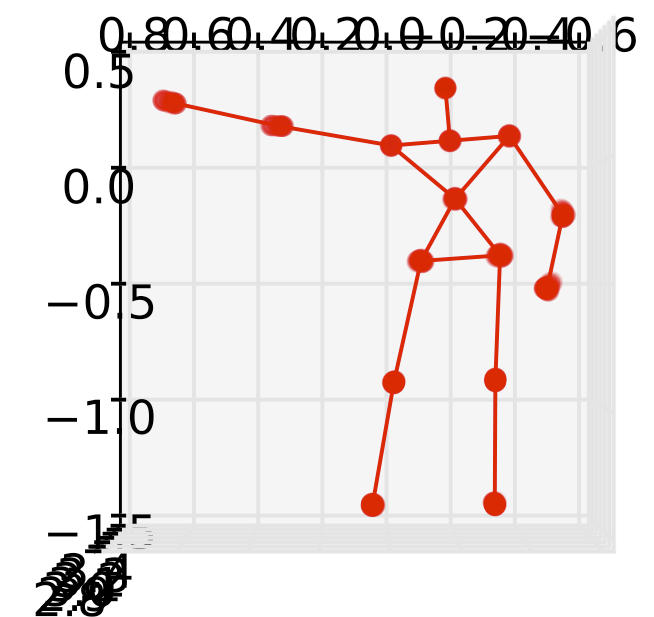
\includegraphics[width=3.5cm]{Figures/right1}} \\
      \hline
      
      RIGHT & Pointing & 4,9,10,22,24 & \parbox[c]{1em}{
      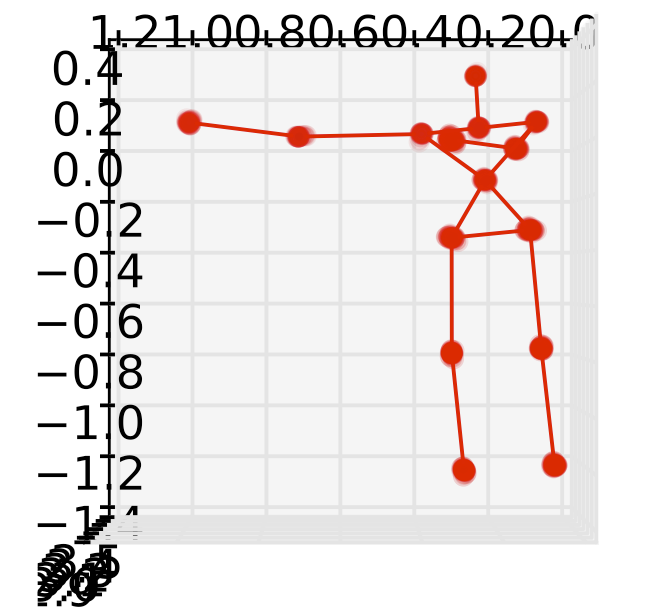
\includegraphics[width=3.5cm]{Figures/right2}} \\
      \hline
      
      LEFT & Pointing & 3 & \parbox[c]{1em}{
      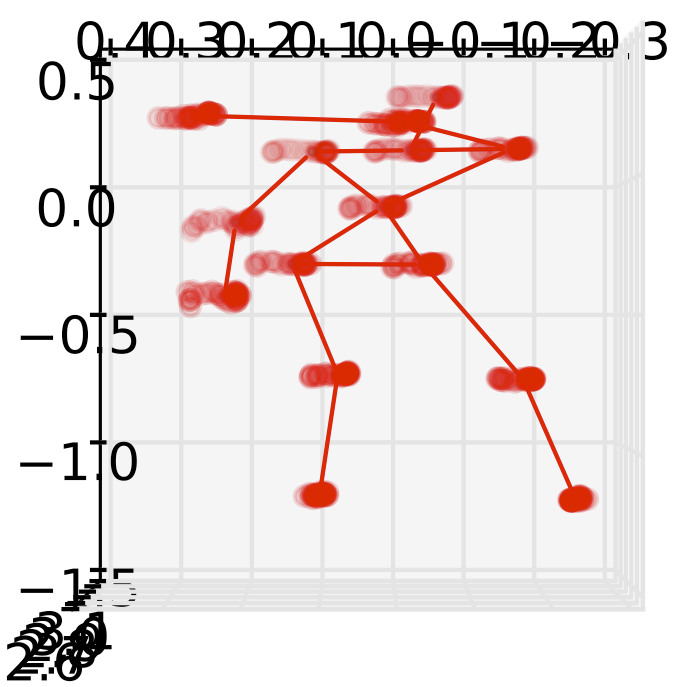
\includegraphics[width=3.5cm]{Figures/right4}} \\
      \hline    
  \end{tabular}
\end{table}

\begin{table}
  [h] \caption{Users pointing \emph{left}}
  \renewcommand{\arraystretch}{2}
  \begin{tabular}
      {|l|l|p{4cm}|p{4cm}|} \hline Pointing hand  & Other hand & Users & Figure Example \\
      \hline
            
    LEFT & Hanging & 
   1,8,11,12,14,16,17,18,\newline
   19,20,26,27 & \parbox[c]{1em}{
   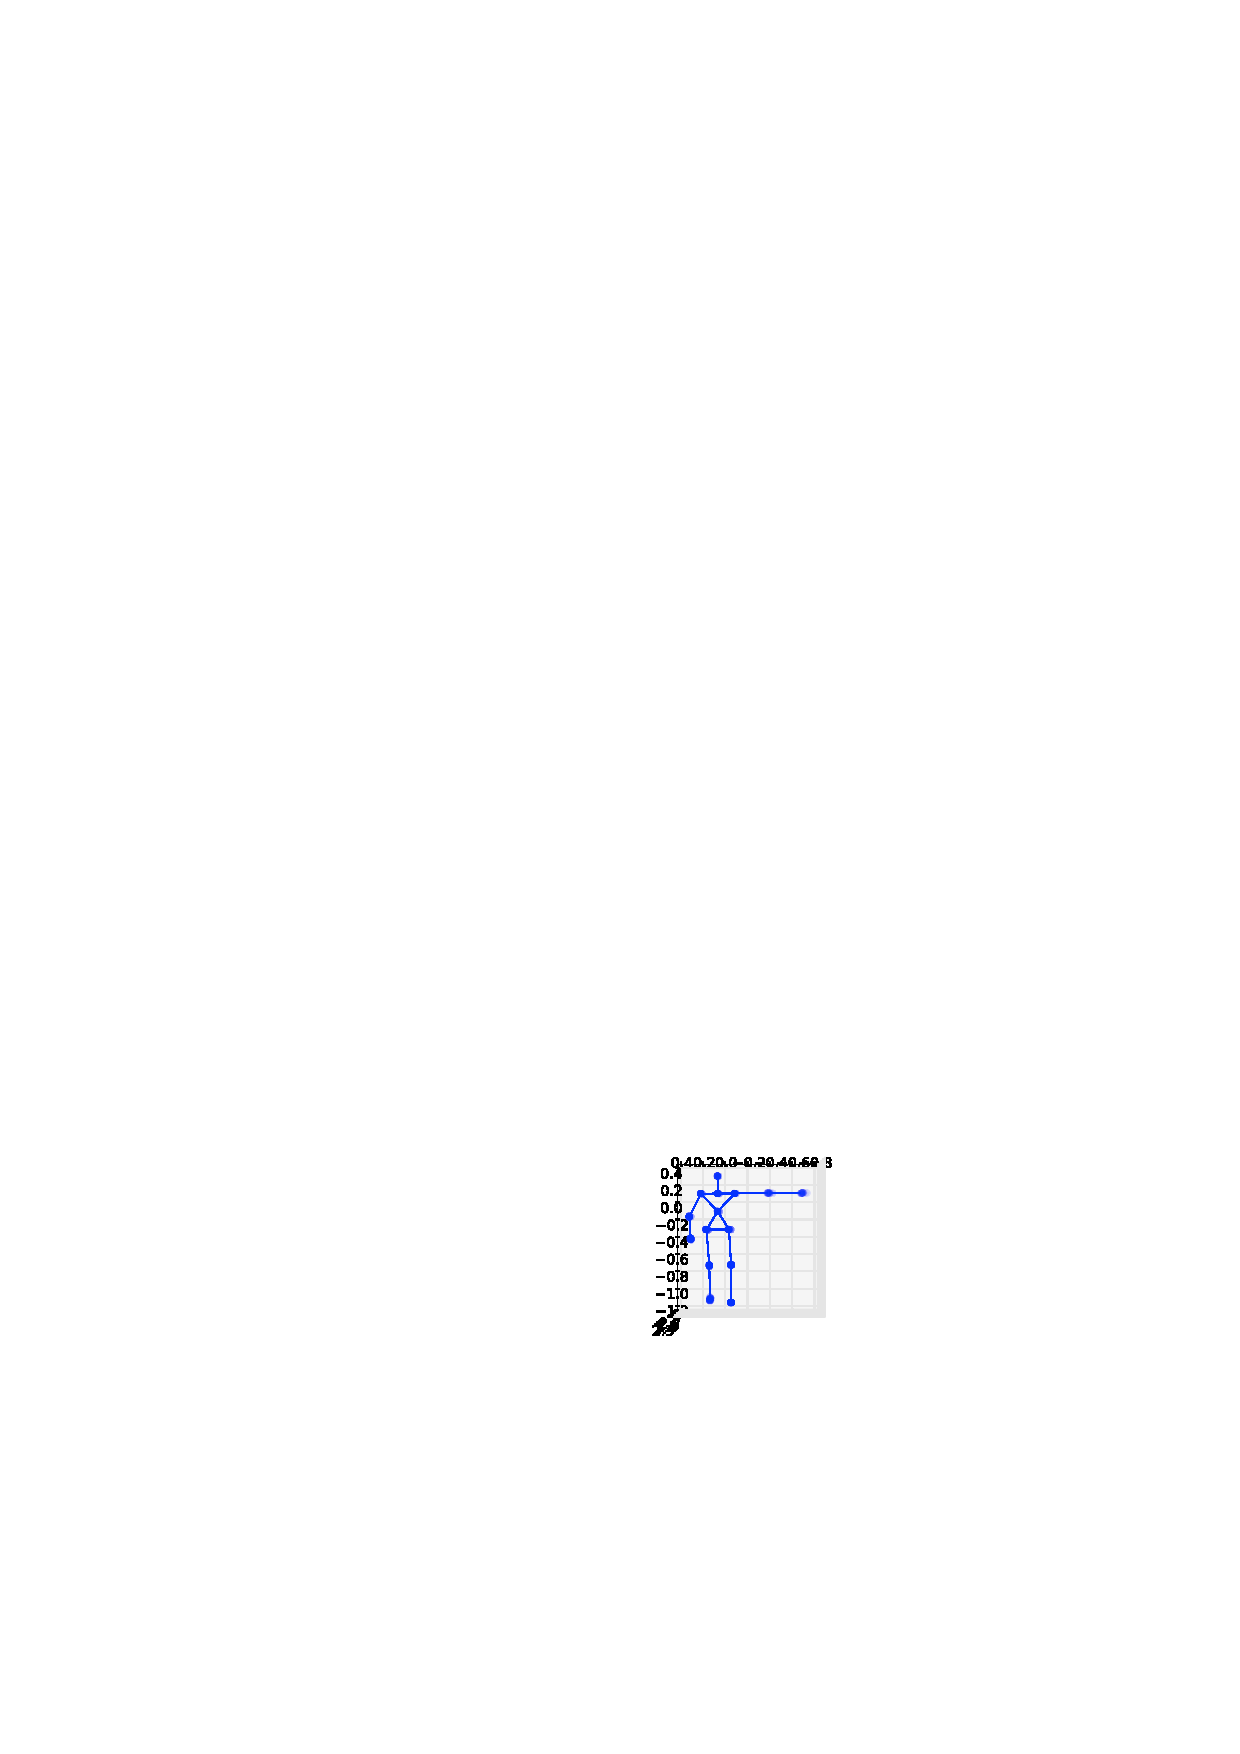
\includegraphics[width=3.5cm]{Figures/left1}} \\
   \hline
          
          
      LEFT & Pointing & 10,13,15,24,25 & \parbox[c]{1em}{
      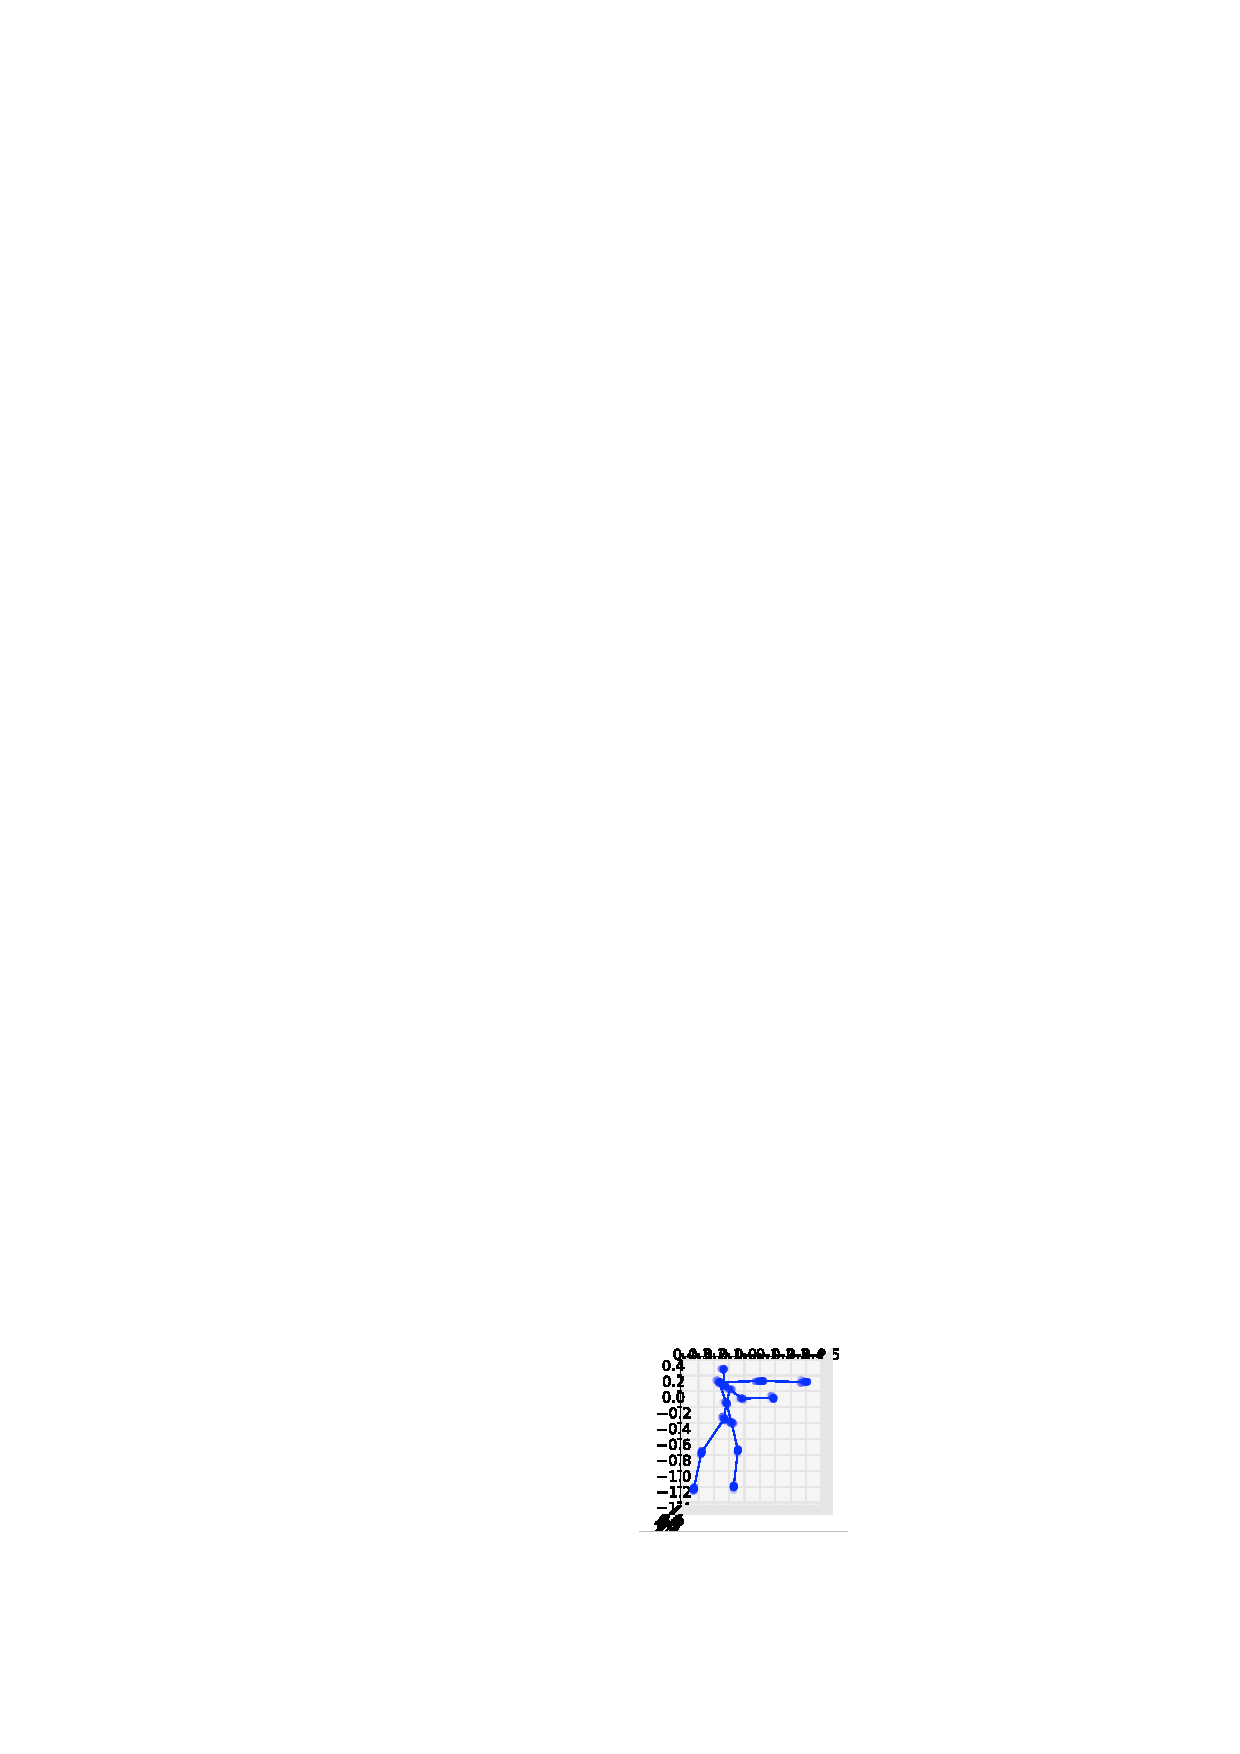
\includegraphics[width=3.5cm]{Figures/left2}} \\
      \hline
          
      RIGHT & Hanging & 2,3,4,5,7,9,21,23, \newline
      28,29,30 & \parbox[c]{1em}{
      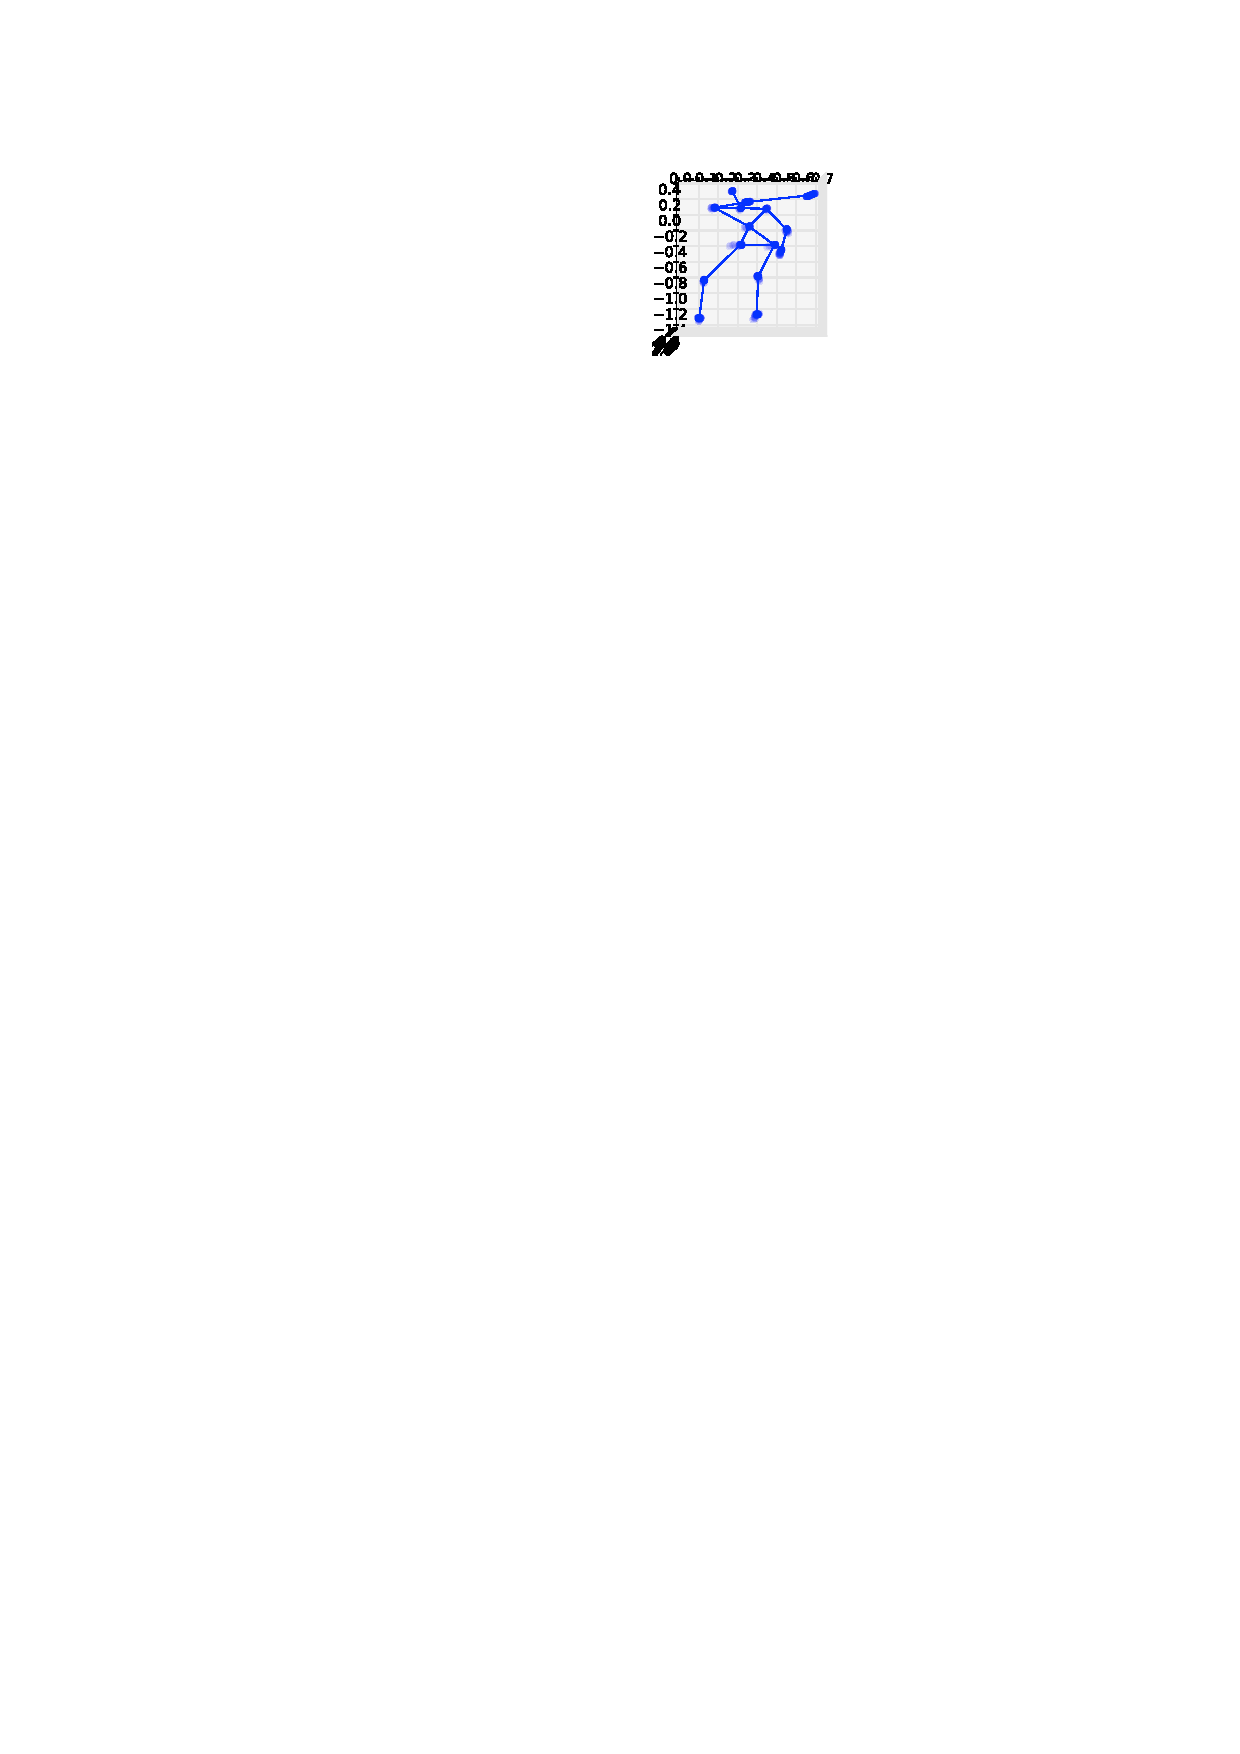
\includegraphics[width=3.5cm]{Figures/left3}} \\
      \hline
      
      RIGHT & Crossed & 22 & \parbox[c]{1em}{
              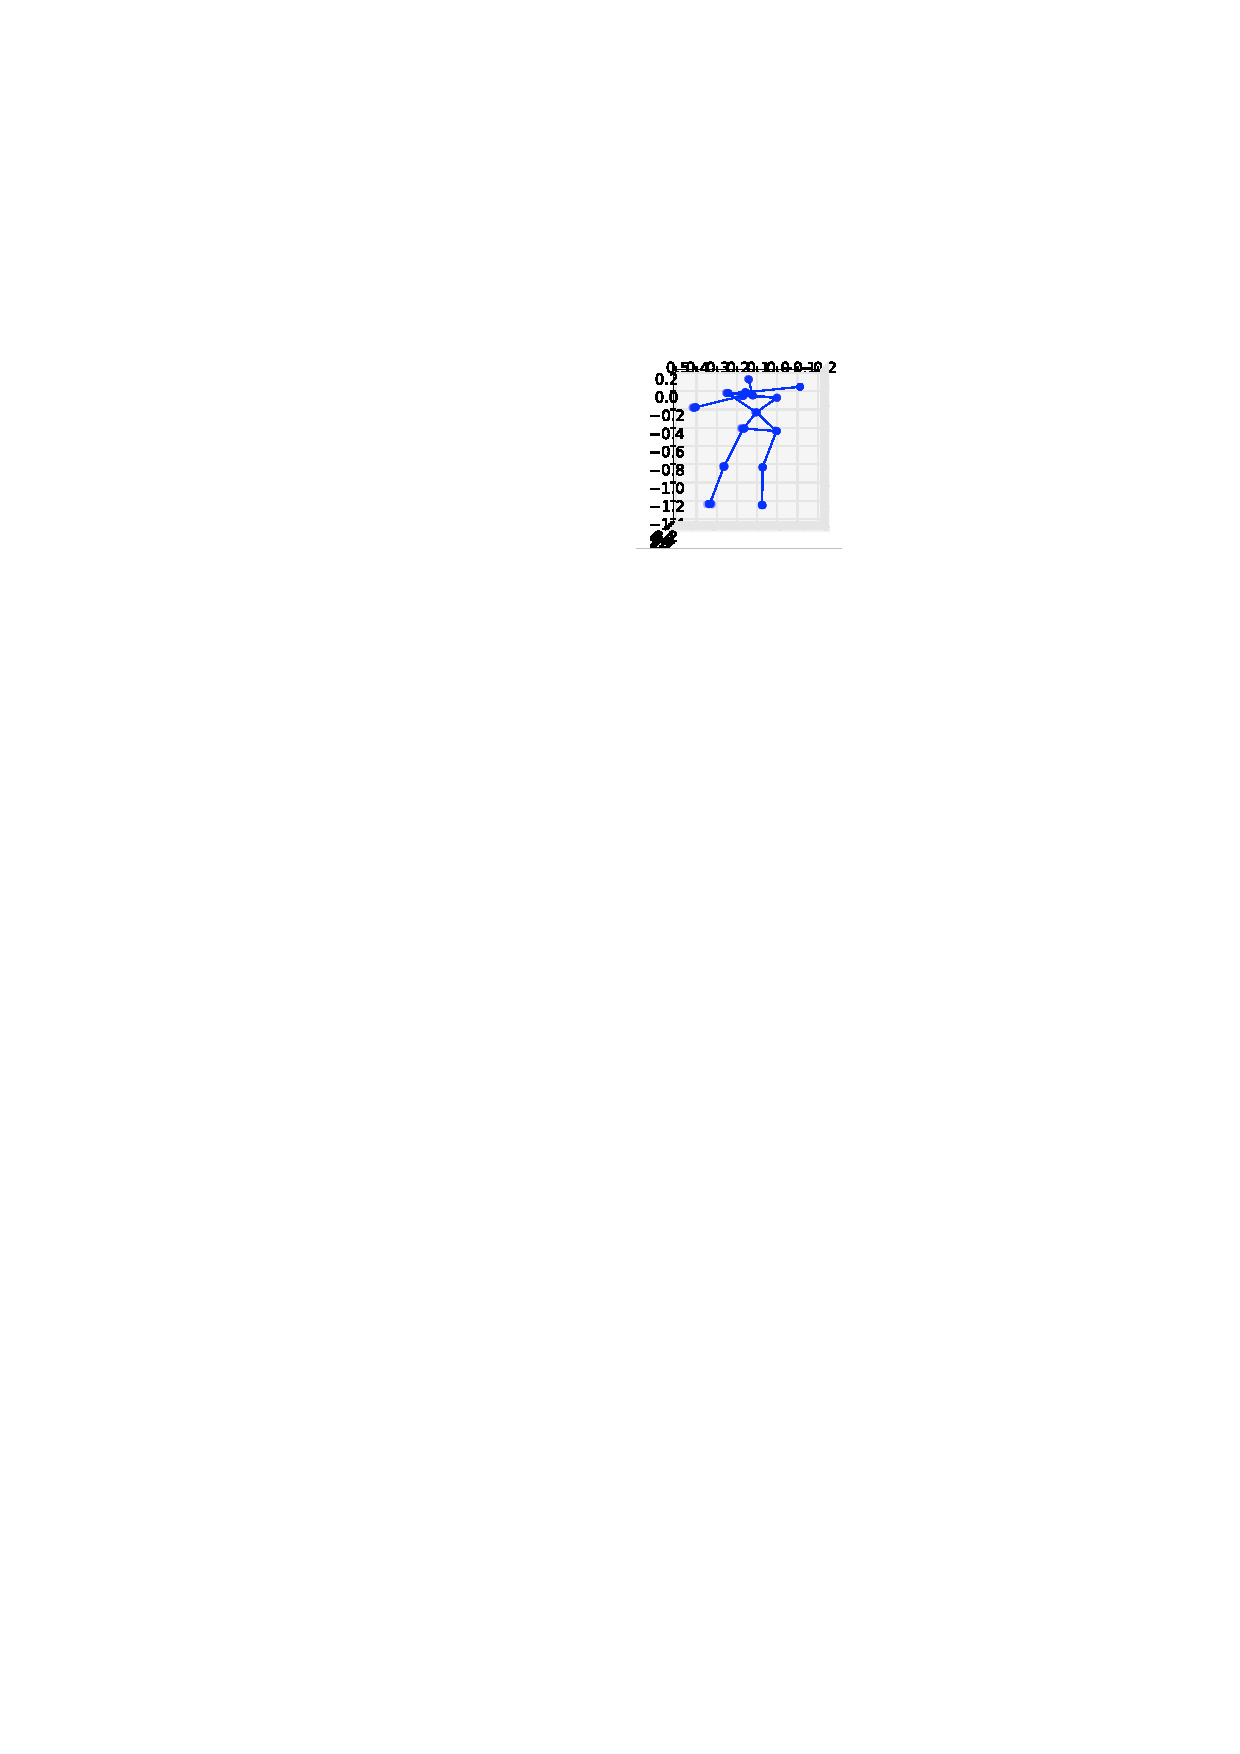
\includegraphics[width=3.5cm]{Figures/left4}} \\
              \hline
  
  \end{tabular}

\end{table}

\begin{table}
  [h] \caption{Users pointing \emph{forward}}
  \renewcommand{\arraystretch}{2}
  \begin{tabular}
      {|l|l|p{4cm}|p{4cm}|} \hline Pointing hand  & Other hand & Users & Figure Example \\
      \hline
            
    LEFT & Hanging & 
   1,8,11,12,17,20 & \parbox[c]{1em}{
   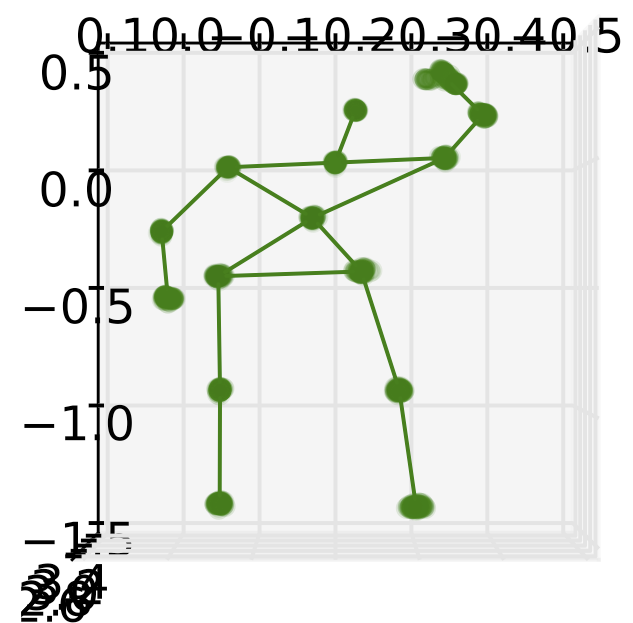
\includegraphics[width=3.5cm]{Figures/forward1}} \\
   \hline
          
          
      RIGHT & Hanging & 2,3,5,7,13,14,15,16,\newline
      18,19,21,23,25,26,27,28, \newline
      29,30 & \parbox[c]{1em}{
      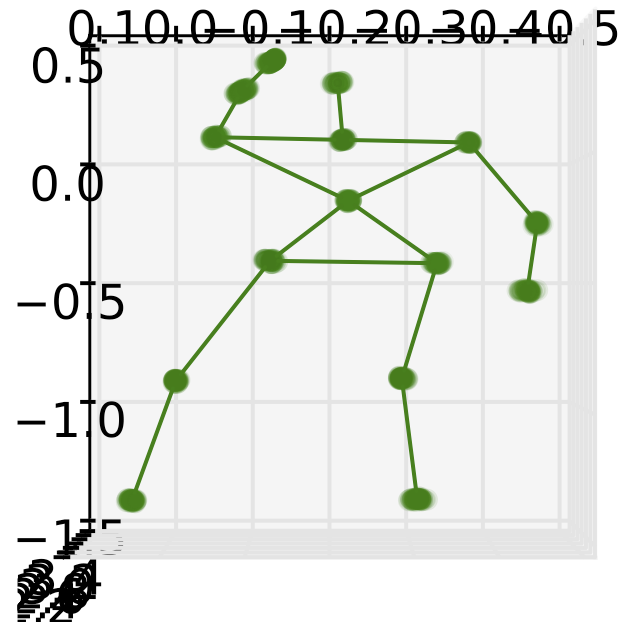
\includegraphics[width=3.5cm]{Figures/forward2}} \\
      \hline
          
      RIGHT & Crossed & 4, 22 & \parbox[c]{1em}{
      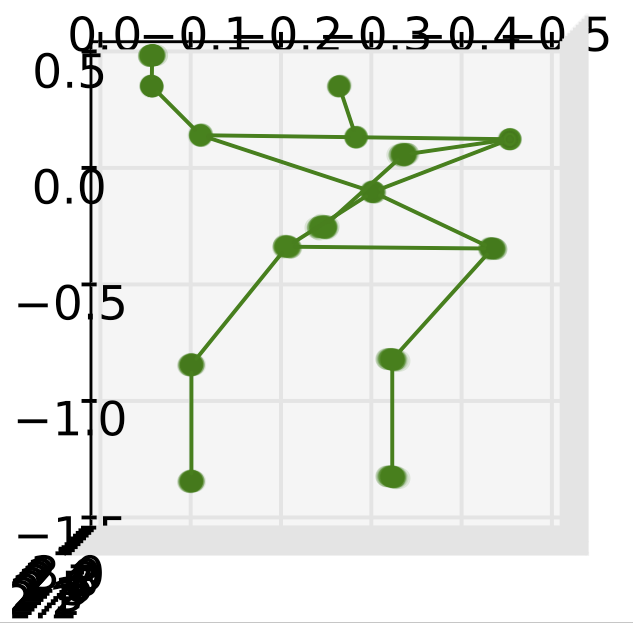
\includegraphics[width=3.5cm]{Figures/forward3}} \\
      \hline
      
      BOTH & - & 10,9,24 & \parbox[c]{1em}{
              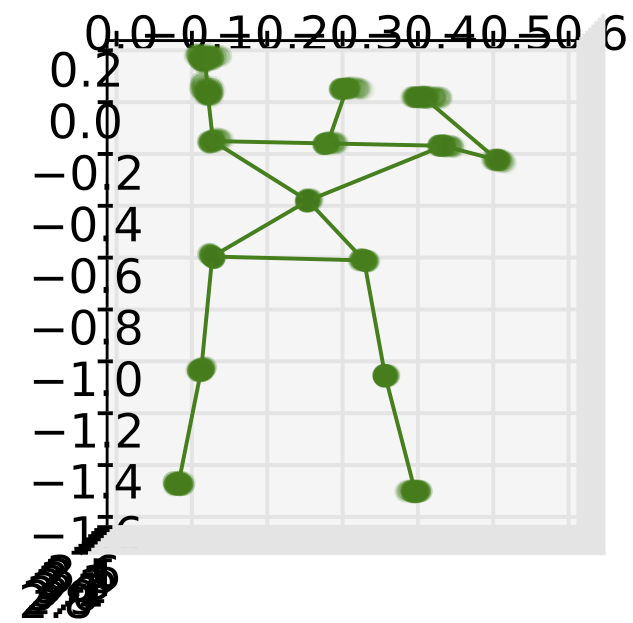
\includegraphics[width=3.5cm]{Figures/forward4}} \\
              \hline

  \end{tabular}

\end{table}

\clearpage

\section{More metrics performed to the experiments}

\label{metrics}

The parameters used to measure the performance were given in terms of Binary classification, and are the following.

\begin{description}
\item[]

\begin{equation}
Precision = \dfrac{TP}{ TP + FP}
\end{equation}

\item[]

\begin{equation}
Recall = \dfrac{TP}{TP + FN}
\end{equation}

\item[]

\begin{equation}
F score = \dfrac{2 \times TP}{2 \times TP+FN+FP}
\end{equation}

\item[]

\begin{equation}
Accuracy = \dfrac{TP + TN}{TP + TN + FP + FN}
\end{equation}

\end{description}

\subsection{Global Novelties}

The following tables expand the performance scores from Table \ref{global}

\begin{table}[!ht]
	\footnotesize
	\renewcommand{\arraystretch}{2}
	\begin{tabular}{p{1.2cm}p{0.7cm}p{0.6cm}p{0.7cm}p{0.7cm}p{0.6cm}p{0.7cm}p{0.7cm}p{0.6cm}p{0.7cm}p{0.7cm}p{0.6cm}p{0.7cm}}
	\hline 
	 & \multicolumn{3}{c}{GMM}& \multicolumn{3}{c}{One class SVM}& \multicolumn{3}{c}{LSA}& \multicolumn{3}{c}{K-means} \\
	 & Mean    & SD & SE& Mean    & SD & SE& Mean    & SD & SE& Mean    & SD & SE \\
	\hline
	Precision  & 0.87 & 0.03 & 0.01 & 0.81 & 0.06 & 0.02 & 0.89 & 0.07 & 0.02 & 0.91 & 0.06 & 0.02      \\
	Recall  & 0.88 & 0.13 & 0.04 & 0.94 & 0.09 & 0.03 & 0.87 & 0.12 & 0.04 & 0.75 & 0.13 & 0.04    \\
	F score  & 0.87 & 0.07 & 0.02 & 0.87 & 0.06 & 0.02 & 0.87 & 0.05 & 0.02 & 0.81 & 0.08 & 0.03    \\ 
	Accuracy   & 0.88 & 0.06 & 0.02 & 0.85 & 0.06 & 0.02 & 0.87 & 0.04 & 0.01 & 0.83 & 0.06 & 0.02   \\
	\hline
	\end{tabular}
	\centering
	\caption[Novelty Detection perfomance for \emph{pointing right} entries]{Novelty Detection performance of the different algorithms when detecting a new entry with a base of knowledge of \emph{pointing right} entries. $ K_{GMM} $ = 3, $ K_{Kmeans} $=1. Note: SD = Standard Deviation, SE = Standard Error  }
\end{table}

If we are interested in having a low recall rate, so we don't bother the user with false alarms, the most appropriate would be One class SVM. On the other hand, if we are interested in precision and don't worry about bothering the user too much, the most precise algorithm would be K-means.


\begin{table}[!ht]
	\footnotesize
	\renewcommand{\arraystretch}{2}
	\begin{tabular}{p{1.2cm}p{0.7cm}p{0.6cm}p{0.7cm}p{0.7cm}p{0.6cm}p{0.7cm}p{0.7cm}p{0.6cm}p{0.7cm}p{0.7cm}p{0.6cm}p{0.7cm}}
	\hline
	 & \multicolumn{3}{c}{GMM}& \multicolumn{3}{c}{One class SVM}& \multicolumn{3}{c}{LSA}& \multicolumn{3}{c}{K-means} \\
	 & Mean    & SD & SE& Mean    & SD & SE& Mean    & SD & SE& Mean    & SD & SE \\
	\hline
	Precision  & 0.72 & 0.10 & 0.03 & 0.70 & 0.06 & 0.02 & 0.77 & 0.40 & 0.13 & 0.69 & 0.34 & 0.11      \\
	Recall  & 0.94 & 0.13 & 0.04 & 0.74 & 0.14 & 0.05 & 0.16 & 0.17 & 0.06 & 0.15 & 0.07 & 0.02    \\
	F score  & 0.80 & 0.04 & 0.01 & 0.72 & 0.09 & 0.03 & 0.24 & 0.21 & 0.07 & 0.24 & 0.10 & 0.03    \\
	Accuracy   & 0.77 & 0.04 & 0.01 & 0.72 & 0.08 & 0.03 & 0.57 & 0.08 & 0.03 & 0.54 & 0.05 & 0.02   \\
	\hline
	\end{tabular}
	\centering
	\caption[Novelty Detection perfomance for \emph{pointing left} entries]{Novelty Detection performance of the different algorithms when detecting a new entry with a base of knowledge of \emph{pointing left} entries. $ K_{GMM} $ = 3, $ K_{Kmeans} $=1. Note: SD = Standard Deviation, SE = Standard Error  }
\end{table}


\begin{table}[!ht]
	\footnotesize
	\renewcommand{\arraystretch}{2}
	\begin{tabular}{p{1.2cm}p{0.7cm}p{0.6cm}p{0.7cm}p{0.7cm}p{0.6cm}p{0.7cm}p{0.7cm}p{0.6cm}p{0.7cm}p{0.7cm}p{0.6cm}p{0.7cm}}
	\hline
	 & \multicolumn{3}{c}{GMM}& \multicolumn{3}{c}{One class SVM}& \multicolumn{3}{c}{LSA}& \multicolumn{3}{c}{K-means} \\
	 & Mean    & SD & SE& Mean    & SD & SE& Mean    & SD & SE& Mean    & SD & SE \\
	\hline
	Precision  & 0.86 & 0.08 & 0.03 & 0.84 & 0.10 & 0.03 & 0.91 & 0.11 & 0.04 & 0.32 & 0.40 & 0.13       \\
	Recall  &  0.96 & 0.07 & 0.02 & 0.77 & 0.19 & 0.06 & 0.37 & 0.17 & 0.06 & 0.15 & 0.19 & 0.06    \\
	F score  & 0.90 & 0.04 & 0.01 & 0.78 & 0.12 & 0.04 & 0.50 & 0.17 & 0.06 & 0.20 & 0.26 & 0.09     \\
	Accuracy   & 0.89 & 0.05 & 0.02 & 0.80 & 0.07 & 0.02 & 0.66 & 0.08 & 0.03 & 0.55 & 0.08 & 0.03   \\
	\hline
	\end{tabular}
	\centering
	\caption[Novelty Detection perfomance for \emph{pointing forward} entries]{Novelty Detection performance of the different algorithms when detecting a new entry with a base of knowledge of \emph{pointing forward} entries. $ K_{GMM} $ = 3, $ K_{Kmeans} $=1. Note: SD = Standard Deviation, SE = Standard Error  }
\end{table}

\clearpage

\subsection{In-class Novelties}

The following tables expand the performance scores from Table \ref{inclass}

\begin{table}[!ht]
	\footnotesize
	\renewcommand{\arraystretch}{2}
	\begin{tabular}{p{1.2cm}p{0.7cm}p{0.6cm}p{0.7cm}p{0.7cm}p{0.6cm}p{0.7cm}p{0.7cm}p{0.6cm}p{0.7cm}p{0.7cm}p{0.6cm}p{0.7cm}}
	\hline 
	 & \multicolumn{3}{c}{GMM}& \multicolumn{3}{c}{One class SVM}& \multicolumn{3}{c}{LSA}& \multicolumn{3}{c}{K-means} \\
	 & Mean    & SD & SE& Mean    & SD & SE& Mean    & SD & SE& Mean    & SD & SE \\
	\hline
	Precision  & 0.90 & 0.12 & 0.04 & 0.63 & 0.10 & 0.03 & 0.95 & 0.11 & 0.04 & 0.73 & 0.14 & 0.05       \\
	Recall  & 0.95 & 0.08 & 0.03 & 1.00 & 0.00 & 0.00 & 0.95 & 0.08 & 0.03 & 1.00 & 0.00 & 0.00    \\
	F score  & 0.92 & 0.07 & 0.02 & 0.77 & 0.08 & 0.03 & 0.95 & 0.07 & 0.02 & 0.84 & 0.09 & 0.03    \\
	Accuracy   & 0.91 & 0.08 & 0.03 & 0.69 & 0.12 & 0.04 & 0.94 & 0.08 & 0.03 & 0.79 & 0.14 & 0.05   \\
	\hline
	\end{tabular}
	\centering
	\caption[Novelty Detection perfomance for \emph{pointing left}, pointing hand \emph{left} other hand \emph{hanging} entries]{Detection performance of the different algorithms when detecting a new entry with a base of knowledge of \emph{pointing left}, pointing hand \emph{left} other hand \emph{hanging}  entries. $ K_{GMM} $ = 30, $ K_{Kmeans} $=1 .Note: SD = Standard Deviation, SE = Standard Error}
\end{table}

\begin{table}[!ht]
	\footnotesize
	\renewcommand{\arraystretch}{2}
	\begin{tabular}{p{1.2cm}p{0.7cm}p{0.6cm}p{0.7cm}p{0.7cm}p{0.6cm}p{0.7cm}p{0.7cm}p{0.6cm}p{0.7cm}p{0.7cm}p{0.6cm}p{0.7cm}}
	\hline 
	 & \multicolumn{3}{c}{GMM}& \multicolumn{3}{c}{One class SVM}& \multicolumn{3}{c}{LSA}& \multicolumn{3}{c}{K-means} \\
	 & Mean    & SD & SE& Mean    & SD & SE& Mean    & SD & SE& Mean    & SD & SE \\
	\hline
	Precision  & 0.62 & 0.14 & 0.05 & 0.58 & 0.08 & 0.03 & 0.78 & 0.39 & 0.13 & 0.86 & 0.18 & 0.06       \\
	Recall  & 0.92 & 0.11 & 0.04 & 0.95 & 0.08 & 0.03 & 0.22 & 0.15 & 0.05 & 0.52 & 0.19 & 0.06    \\
	F score  & 0.73 & 0.08 & 0.03 & 0.72 & 0.07 & 0.02 & 0.32 & 0.20 & 0.07 & 0.62 & 0.16 & 0.05    \\
	Accuracy   & 0.64 & 0.12 & 0.04 & 0.62 & 0.12 & 0.04 & 0.60 & 0.06 & 0.02 & 0.71 & 0.10 & 0.03   \\
	\hline
	\end{tabular}
	\centering
	\caption[Novelty Detection perfomance for \emph{pointing left}, pointing hand \emph{right} other hand \emph{hanging} entries]{Detection performance of the different algorithms when detecting a new entry with a base of knowledge of \emph{pointing left}, pointing hand \emph{right} other hand \emph{hanging} entries. $ K_{GMM} $ = 30, $ K_{Kmeans} $=1.Note: SD = Standard Deviation, SE = Standard Error}
\end{table}


\begin{table}[!ht]
	\footnotesize
	\renewcommand{\arraystretch}{2}
	\begin{tabular}{p{1.2cm}p{0.7cm}p{0.6cm}p{0.7cm}p{0.7cm}p{0.6cm}p{0.7cm}p{0.7cm}p{0.6cm}p{0.7cm}p{0.7cm}p{0.6cm}p{0.7cm}}
	\hline 
	 & \multicolumn{3}{c}{GMM}& \multicolumn{3}{c}{One class SVM}& \multicolumn{3}{c}{LSA}& \multicolumn{3}{c}{K-means} \\
	 & Mean    & SD & SE& Mean    & SD & SE& Mean    & SD & SE& Mean    & SD & SE \\
	\hline
	Precision  & 0.67 & 0.13 & 0.04 & 0.57 & 0.09 & 0.03 & 0.79 & 0.30 & 0.10 & 0.60 & 0.25 & 0.08       \\
	Recall  & 0.80 & 0.18 & 0.06 & 0.88 & 0.15 & 0.05 & 0.50 & 0.25 & 0.08 & 0.53 & 0.27 & 0.09    \\
	F score  & 0.71 & 0.13 & 0.04 & 0.69 & 0.10 & 0.03 & 0.58 & 0.23 & 0.08 & 0.54 & 0.22 & 0.07    \\
	Accuracy   & 0.68 & 0.15 & 0.05 & 0.60 & 0.12 & 0.04 & 0.69 & 0.11 & 0.04 & 0.62 & 0.11 & 0.04   \\
	\hline
	\end{tabular}
	\centering
	\caption[Novelty Detection perfomance for emph{pointing forward}, pointing hand \emph{right} other hand \emph{hanging} entries]{Detection performance of the different algorithms when detecting a new entry with a base of knowledge of \emph{pointing forward}, pointing hand \emph{right} other hand \emph{hanging} entries. $ K_{GMM} $ = 30, $ K_{Kmeans} $=1. Note: SD = Standard Deviation, SE = Standard Error}
\end{table}

\begin{flushright}

\end{flushright}